\begin{abstract}
 Ce document est rédigé dans le cadre de la première année d'alternance de Lucas Sovre au sein de \acrshort{edf} R\&D, en partenariat avec l'école ESIEE-IT.
 Mon tuteur entreprise est un ingénieur chercheur : Julien Caron. Bien que ce rapport ne présente pas de données confidentielles, sa diffusion doit rester réduite.
\end{abstract}
\chapter{Présentation de EDF.}
\section{L'histoire de EDF.}
Dans les années 30, deux cents entreprises privées assurent la production, une centaine le transport et plus de mille la distribution de l’électricité. L’approvisionnement et les tarifs de l’électricité sont alors très différents selon les prestataires et les régions.Après-guerre, la création d’un service public unique de l’électricité devient alors une nécessité. La première tâche du groupe \acrshort{edf} est de reconstruire entièrement le réseau de transport partiellement détruit pendant la guerre et de relancer la construction de grands ouvrages hydrauliques dont certains avait été interrompu par la guerre. De 1946 à 1970, la France achète à l’étranger 76\% de son approvisionnement en énergie et le pétrole constitue 84\% de ces importations. Dès 1973, à la suite de la crise pétrolière, la France se tourne vers la production d’électricité à partir d’énergie nucléaire et annonce la construction des 13 premières centrales entre 1974 et 1975, avec une volonté : garantir son indépendance énergétique.

Avec les années, \gls{edf} acquiert une expertise, un savoir-faire technologique et des compétences de haut niveau, et s’impose comme un leader mondial dans le domaine de l’énergie.

A la fin du siècle dernier, le marché de l’électricité s’ouvre à la concurrence et \acrshort{edf} se développe en Europe et à l’international. Les échanges s’intensifient, ainsi que la prise en compte des problématiques de développement durable. \acrshort{edf} lance le chantier d’une centrale nucléaire de nouvelle génération à Flamanville. La construction de ce premier EPR en France (réacteur pressurisé européen) est une étape essentielle dans la préparation du renouvellement du parc nucléaire d’\acrshort{edf}.

\section{Fonctionnement d'une centrale nucléaire.}

Une centrale nucléaire REP (Réacteur à Eau Préssurisée) repose sur la fission nucléaire afin de transformer de l’énergie nucléaire en énergie électrique. On trouve dans le cœur du réacteur nucléaire le matériau fissible, dans notre cas il s’agit de l’uranium 235, on va déclencher dans celui-ci une réaction en chaine de façons à produire de l’énergie thermique et ainsi chauffer l’eau du circuit primaire circulant dans la cuve du réacteur. Elle est à 325 °C mais reste liquide grâce au pressuriseur qui maintient le circuit primaire à 155 Bar. L’eau sortant de la cuve va passer dans le faisceau tubulaire de chaque générateur de vapeur afin de pouvoir léguer son énergie thermique à l’eau du circuit secondaire. Celle-ci en circulant dans les GV va se transformer en vapeur pour alimenter le groupe turbo alternateur comprenant une turbine et un alternateur.

La turbine est constituée d'un corps haute pression (HP) et de plusieurs corps basse pression (BP), après passage dans le corps HP, la vapeur passe ensuite dans les générateurs sécheurs surchauffeurs (GSS) afin d’améliorer son titre avant d'alimenter les corps BP. Les turbines BP et la turbine HP se trouvent sur le même arbre donc elles tournent à la même vitesse et entraînent un alternateur qui produit l'électricité. La vapeur est ensuite condensée en eau puis envoyée vers les GV au travers du poste d'eau qui permet d'améliorer le rendement de l'installation. Le condenseur, lui va être refroidi par un troisième circuit lié au fleuve passant près de la centrale ou par des aéroréfrigérants.

Il est important de noter que les fluides des circuits primaire, secondaire et de refroidissement échangent de l’énergie entre eux mais ne sont en aucun cas en contact. Ces trois circuits sont strictement indépendants les uns des autres.

\centering{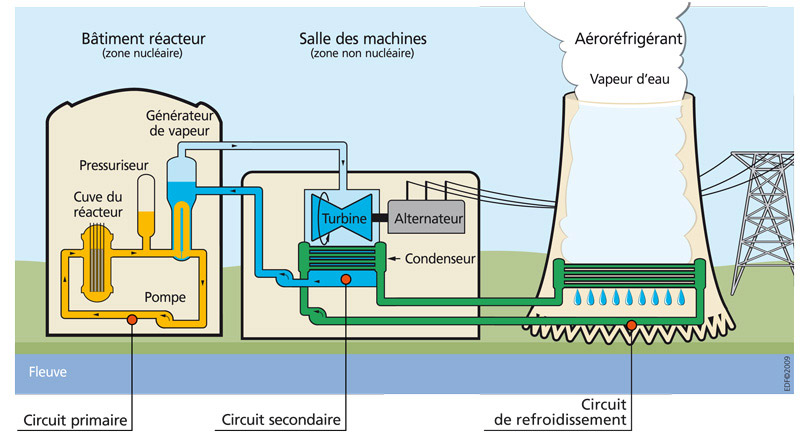
\includegraphics[scale=0.44]{images/schemaREP.jpg}}

~\cite[IRSN]{IRSN_rep_schema}

\justify
\section{La recherche et développement}

\subsection{Présentation de la R\&D}

La R\&D est au cœur d’enjeux majeurs du Groupe \acrshort{edf}. Elle couvre l’ensemble des métiers et activités du secteur de l’énergie. Elle appuie au quotidien les métiers et les filiales en cohérence avec le projet du Groupe \acrshort{edf}, Cap 2030. Deux missions animent les chercheurs : améliorer la performance dans toutes les activités d’aujourd’hui et préparer l’avenir en travaillant sur les technologies de rupture.

En quelques chiffres \acrshort{edf} R\&D c'est 518 Millions d'euro de budget, 160 doctorants, 1800 salariés et 11 pétaflops de capacité de calcul (en 2020).

\subsection{Mon environnement de travail au sein de la R\&D}
Je travaille sur le site de \acrshort{edf} lab Paris-Saclay, qui est situé au coeur du plateau universitaire de Saclay. Ses activités et domaines de recherche sont trés diversifiés : mécanique vibratoire, génie logiciel, mathématiques et simulation numérique, économie de l'électricité, management des risques industriels, NTIC et architectures de comptage et digitales, traitement des méga-données, relation client et création de nouveaux services...

Je travaille au sein du département Pericles, dans le groupe I2A. Il est spécialisé dans l' architecture informatique.

\textit{
 "En informatique, architecture désigne la structure générale inhérente à un système informatique, l'organisation des différents éléments du système (logiciels et/ou matériels et/ou humains et/ou informations) et des relations entre les éléments. Cette structure fait suite à un ensemble de décisions stratégiques prises durant la conception de tout ou partie du système informatique, par l'exercice d'une discipline technique et industrielle du secteur de l'informatique dénommée elle aussi architecture, et dont le responsable est l'architecte informatique."
} \cite{wikipedia_archi_info}

Mes collègues sont essentiellement des ingénieurs chercheurs et mon travail consiste à participer aux projets de façons active pendant toutes les phases : 
\begin{itemize}
\item Caractérisation des besoins.
\item Prototypage d'un "\gls{POC}".
\item Décision des choix architecturaux.
\item Développement de la solution.
\item Prise en compte du retour client.
\end{itemize}

\chapter{Mes projets.}
\section{Projet ARDEN}
\subsection{Contexte}
Les centrales nucléaires francaises s'appuient sur de multiples systèmes de sécurités pour garantir une exploitation en toute sureté. L'un des principaux éléments de ce système est l'enceinte du réacteur nucléaire, plus communément appelé \acrshort{br} (Batiment Réacteur).

\textit{"Le bâtiment réacteur (ou enceinte de confinement) [...] assure le confinement des substances radioactives par rapport à l’environnement extérieur et la protection du réacteur contre les agressions externes. 
Le bâtiment réacteur abrite la cuve, le circuit primaire, une partie des circuits secondaires [...]
De manière schématique, le bâtiment du réacteur est constitués d’un cylindre en béton surmonté d’un dôme en béton (toit du bâtiment) qui forme une enveloppe résistante et à étanchéité spécifiée.
[...]Elle est conçue pour résister à la pression atteinte lors des accidents retenus à la conception du réacteur (4 à 5 bars absolus) et pour rester étanche dans ces circonstances. Les parois en béton reposent sur un radier lui-même en béton qui constitue le socle du bâtiment."} \cite[IRSN]{IRSN_suretee}

Les exploitants de tout \acrshort{cnpe} mènent réguliérement des essais afin d'assurer une disponibilité maximum de ses organes de sureté. 

Dans ce cadre, lors de chaque \gls{VD}, des essais sont menés sur le \acrshort{br}. Notamment une épreuve d'étanchéité au cours de laquelle le \gls{br} est monté en pression à 5 bar , soit environ 5 fois la pression atmosphérique (1 atm = 1.013 bar).

Les essais menés sont alors source de nombreuses données essentielles.

La R\&D de \gls{edf} a décidé de mener des recherches pouvant prédire le comportement du vieillissement des reacteurs nucléaires. Pour cela une réplique exacte à l'échelle 1/3 à été créee. Grâce à divers procédés physico-chimiques celle-ci viellit neuf fois plus vite que les batiments réacteurs nucléaires du parc français. Ainsi en reproduisant le cycle de vie des vrais CNPE sur ce \gls{br}. Les données générées lors des \gls{VD} sur cette réplique nous permettent de prédire précisément l'évolution des \gls{br} en production.

Lors de ces expérimentations la grande quantité de données générées nécéssitent un système d'informations robuste et pérenne.
\subsubsection{Caractérisation du besoin.}

Par analogie avec le Carnet de Santé, le système ARDEN a pour objectif d’être le référentiel des informations connues sur les enceintes, organisées dans le temps par la séquence des événements majeurs (construction, mise en service, visites de contrôle, travaux d’inspection, travaux de réparation), puis dans l’espace au moyen d’une partition géométrique du bâtiment en Zones Fonctionnelles.

La modélisation scientifique et la simulation numérique peuvent alors venir aider le médecin à mieux comprendre les mécanismes à l’œuvre (séchage et fluage qui déterminent la dégradation de l’enceinte), puis dans une certaine mesure prévoir l’évolution et proposer des remédiations (prédiction de fuite et analyse des scénarios de recouvrement des compléments d’étanchéité).

\centering{
 \fbox{
  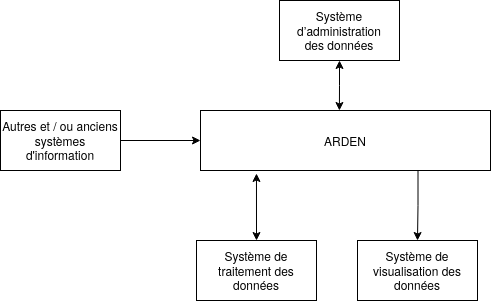
\includegraphics[scale=0.5]{images/ARDEN_generalNeed.png}
 }
}

\justify
\subsection{Notre environnement de développement et méthode de travail.}

Nous sommes principalement 3 ingénieurs chercheurs à travailler sur ce projet. Nous avons fait le choix de ne pas choisir d' \textit{\gls{ide}}. Afin de ne pas nous bloquer avec une technologie propriétaire. Néamoins, nous avons fait me choix d'utiliser Gradle pour la compilation du java. C'est un moteur open source de compilation Java, Scala, C++ et Groovy. Un de ses attraits (en plus de ses hautes performances), est sa facilité de prise en main.

Afin de travailler efficacement sur le même projet, nous utilisons un outil de gestion de version de code : Gitlab.
Cela nous permet de travailler sur les mêmes portions de code sans être intrusif sur le travail des autres.
Gitlab nous à également permis de mettre en place une dynamique d'intégration continue : cela nous permet de déclencher une serie d'actions automatique lorsque nous poussons notre travail sur Gitlab. (voir schéma ci-dessous, également disponible en annexe 2).

\centering{
 \fbox{
  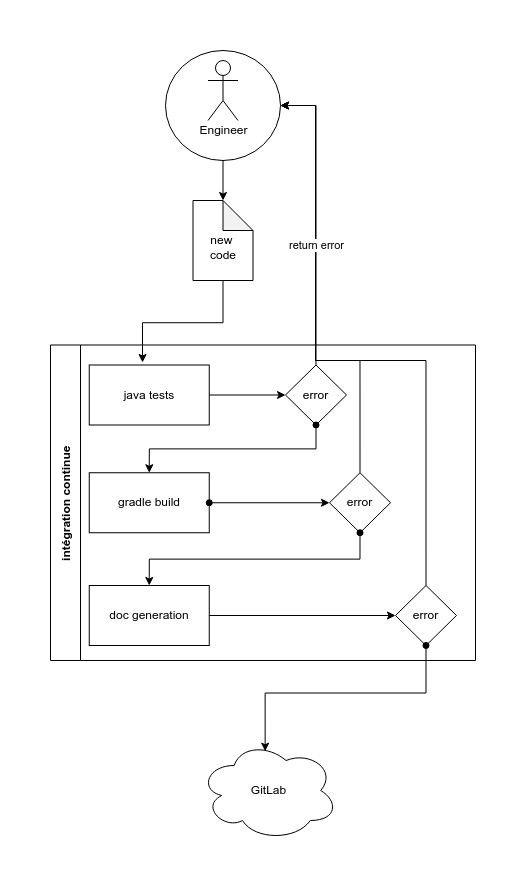
\includegraphics[scale=0.4]{images/CI_CD.png}
 }
}

\justify

Ce système d'intégration permet de prévenir l'envoi de code erronné en production car il est ainsi systématiquement testé.

\justify
\subsection{Choix d'architecture informatique.}

\subsubsection{Choix de l'interface d'accès au système.}

Le système ARDEN sera accessible sous forme d'\gls{api} \gls{rest}. Ce choix est motivé par le fait que l' API RESTful est un standard de l'industrie permettant de facilement déployer le système sous forme d'architecture microServices. De plus, la forme standard des \gls{api} \gls{rest} facilite grandement les intégrations avec d'autres systèmes.

\begin{minipage}{0.90\textwidth}
 \underline{
  Les \gls{api} \gls{rest} :
 }
 L'architecture REST a été créée par l'informaticien Roy Fielding en 2000 dans sa thèse de doctorat Architectural Styles and the Design of Network-based Software Architectures . \cite{REST_theses}
 Dans le cas d'une \gls{api} web RESTful des standard suplémentaires sont appliqués :
 \begin{itemize}
  \item  Architecture serveur-client.
  \item Sans état. (L’API traite chaque requête comme une première demande.)
  \item Mise en cache. (Les données fréquemment demandées sont mises en cache pour réduire la bande passante.)
  \item Interface uniforme. (Méthodes de communication post, get, put, delete)
  \item Possibilité de plusieurs couches.
 \end{itemize}
 Communément une interface \gls{api} \gls{rest} web implémente au minimum les 4 méthodes http par point d'accès (GET, POST, PUT, DELETE). Une cinquième méthode(PATCH) existe mais est parfois confondue avec PUT dans son utilisation. Leur différence est que PATCH permet de mettre à jour uniquement certains champs d'un objects, alors que PUT remplace complétement un object défini par celui envoyé.
\end{minipage}

\centering{
 \fbox{
 \begin{minipage}{0.90\textwidth}
 \underline{Note :}

 Dans certains cas ne pas donner accès à certaines méthodes HTTP pour certains endpoint peut être un choix délibéré d'architecture afin de limiter les actions d'utilisateurs. 

 \underline{Exemple :} donner uniquement accès à la visualisation des données à certains utilisateurs.
 \end{minipage}
 }
}

\justify
\subsubsection{Choix de la technologie de sauvegarde des données.}

La sauvegarde des données doit être realisée dans une \gls{bdd} car cette technologie permet de centraliser, sécuriser et simplifier les transactions de données.

Il existe dans l'industrie actuelle deux standards principaux en terme de \gls{bdd} :
\begin{itemize}
 \item \gls{bdd} relationnelle (SQL ou SGBDR) : Système qui est basé sur une architecture en tables de données.
 \item \gls{bdd} non relationelle (noSQL) : système qui n'a pas d'architecture prédéfinie, qui est basée sur un système de clé-valeur pour lier les objects entre eux. \cite{BDD_theses}
\end{itemize}

Dans le cas du projet ARDEN, le retour d'expérience de cette technologie, les avantages d'évolutivité et de disponibilitée face à de grands nombres de transactions ont porté notre choix sur une \gls{bdd} relationelle.

Dans les bases de données relationnelles de multiples moteurs de \gls{bdd} existent (Postgresql, MySql, Sqlite3 , Oracle Database ...)

Le choix de moteur de \gls{bdd} doit être mené en prenant en compte les propriétés \gls{acid} :
\begin{itemize}
 \item Atomicité : cela assure qu'une transaction soit effectué de facons totale ou aucunement (si une requête de 500 ligne est performée, mais qu'une seule ligne pose problème : la totalité de la transaction est abandonnée). 
 \item Cohérence : toutes les requêtes doivent strictement respecter les règles de la base de données pour être executées.
 \item Isolation : chaque transaction doit s'exécuter en isolation totale : si T1 et T2 s'exécutent simultanément, alors chacune doit demeurer indépendante de l'autre. 
 \item Durabilité : assurer que les données restent intègres dans le temps, sans être altérées par des facteurs extérieurs.
 \cite{wikipedia_acid}
\end{itemize}

Il faut noter que ces propriétés ne sont pas toujours désirées. Selon le besoin l'atomicité peut ne pas être voulue lorsque les requêtes ne sont pas reproductibles et que les données sont cruciales.

Dans notre cas, nous avons choisi Postgresql pour le retour d'expérience positif, sa grande évolutivité et sa polyvalence en terme de propriétés \gls{acid}.
\subsubsection{Choix de technologie de langage logiciel.}

Concernant le langage informatique dans lequel créer le coeur de l'application ARDEN l'ordre des possibles étant assez vaste (nodejs, python, java, C++, .NET, Golang ...). Notre choix s'est orienté grâce au retour d'expérience (pas de technologies émergentes), de la portabilité du langage (exécution indépendante du système d'exploitation.), de sa communautée et de son évolutivité. Mais au delà des aspect techniques, nous devons également prendre en compte "le catalogue des solutions EDF". C'est une liste de logiciels que \gls{edf} utilise couramment et leur utilisations est primordiale pour que les services informatiques d'exploitation puissent le maintenir. 

Le java répond à toutes ces spécifications : 
le \gls{jdk} permet d'assurer une portabilité totale du java. Même s'il a beaucoup évolué depuis, il date de 1995 et possède une des plus grandes communautés de la sphère informatique. Dernièrement, le java est très évolutif. 

Nous avons également fait le choix d'utiliser SpringBoot : il s'agit d'un framework java facilitant le development de logiciels professionnels ortienté web.
Comme exposé precedement (c.f 2.1.2 Notre envirtonement de travail) nous avons également décidé d'utiliser Gradle pour faciliter la compilation, le déploiement et la gestion des dépendances de notre projet.

Concernant l'injection de scripts SQL au démarrage et la migration de bases de données : nous avons choisi d'utiliser Flyway, qui est un outil open-source sans dépendances et sans format ou langage propriétaire.

Nous avons également choisi d'implémenter une génération de documentation Open-API. C'est un standard de l'industrie pour facilement documenter les différentes spécifications d'une \gls{api}.

Nous allons également utiliser un client python sous la forme de paquet pour permettre aux utilisateurs finaux d'appeler l'\gls{api} de façon simple et sans mauvaises utilisations de la base de donnée.

Le schéma ci-dessous résume l' architecture de ce projet (également disponible en annexe 1) : 

\centering{
 \fbox{
  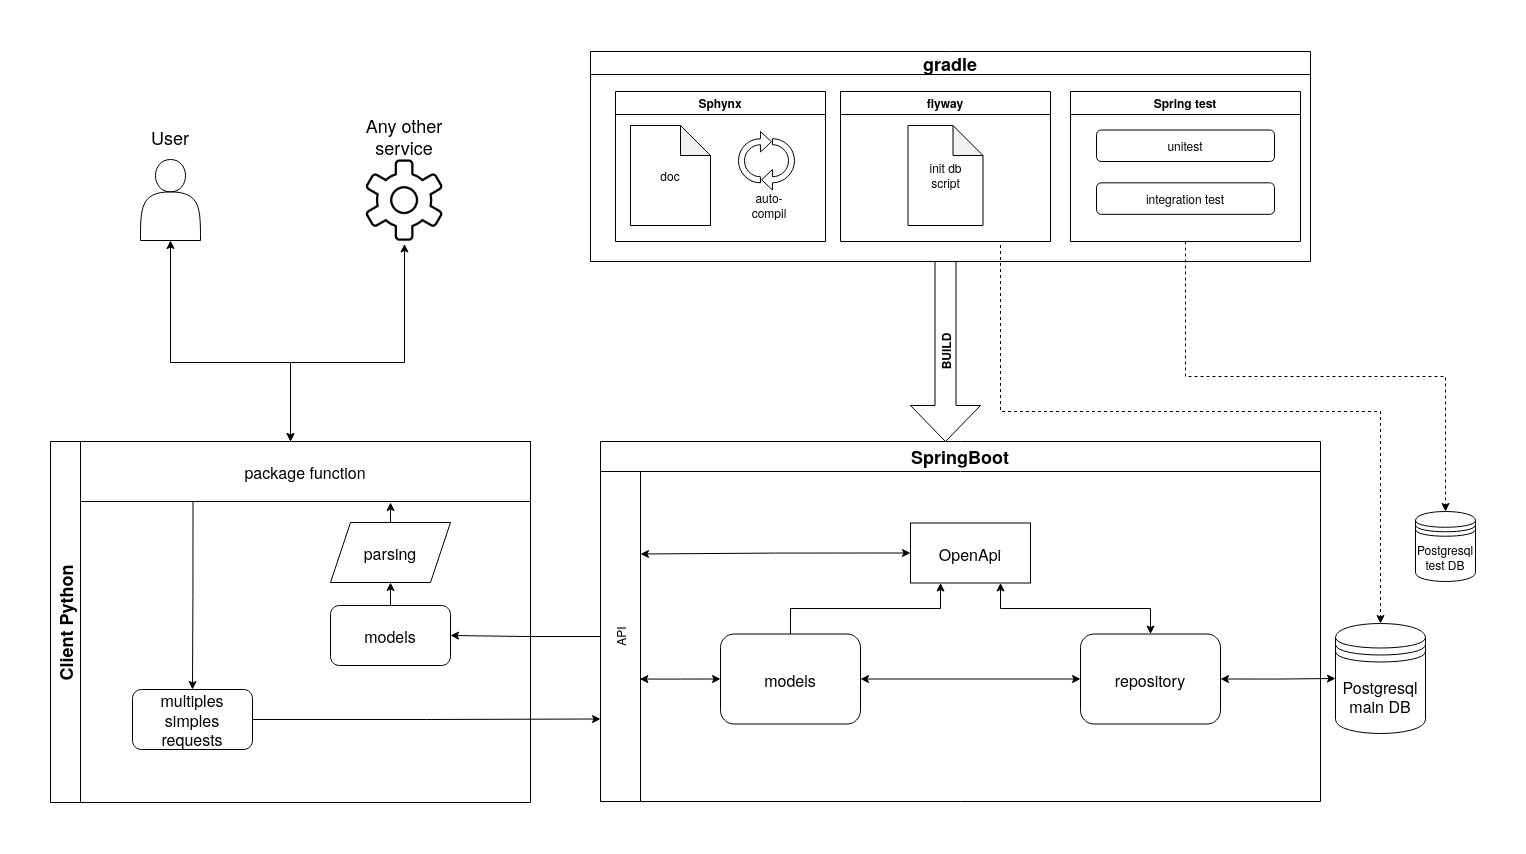
\includegraphics[scale=0.20]{images/ARDEN_techno.png}
 }
}

\justify
\subsection{Etat actuel du projet}

Le principal du travail sur le serveur java est terminé, celui-ci peut être servi sur une instance TomCat. Les principales routes d'accès aux objects en base de données sont fonctionnelles et possèdent leurs tests d'intégration. Seul le système d'authentification utilisateurs n'est pas encore fonctionel et doit être relié à l'annuaire des applications \gls{edf}.

Un client python pour faciliter l'accès à l'API du serveur java est en phase de concéption.

\subsection{Avancement prévu du projet}

D'ici septembre, je devrais avoir participé à la recette d'un logiciel de calculs physiques sous-traités à une autre entreprise.
Prochainement, quand le client python du projet ARDEN sera développé : nous ferons un premier rendu client et entrerons dans une série de rendu/retour client, à la manière d'une méthode agile avant d'arriver à une version 1.0.
\clearpage

\section{Conclusion}

Lors de cette première partie d'alternance, j'ai débuté ma 4ème année consécutive chez \gls{edf}. J'ai découvert le monde de la recherche et developpement, ainsi que les méthodes de travail des ingénieurs chercheurs. Mais j'ai aussi continué à developper ma capacité à travailler en autonomie.

Mais ce que j'ai surtout découvert et retenu de cette période est le plaisir de travailler dans un domaine qui me passione et m'anime profondément. L'architecture informatique est une réelle passion et il me reste tant à apprendre. 

Cette conclusion peut être un peu trop personnelle pour un premier rapport. Mais je ne me permettrais pas de faire de reele conclusion sur cette première année d'alternance avant de l'avoir complément accomplie.